\section{When a Physical Explanation Can Be Distinguished}
\label{sec:narrative-information}

A physical model does not remove an information limit. Two sources can produce nearly the same reports after their amplitudes and initial conditions are allowed to vary. High confidence in the state estimate therefore need not imply high confidence in a source.

The distinction is explicit in a local model. With observation matrix $C$, transition $A$ and requested hidden-voltage map $L$, functional reconstruction requires
\begin{equation}
 \ker\mathcal O_H\subseteq\ker L,\qquad
 \mathcal O_H=\operatorname{col}(C,CA,\ldots,CA^H).
 \label{eq:narrative-functional}
\end{equation}
Unobservable directions are harmless for this target if they do not change $Lx$ \cite{fernando2010functional,montanari2022functional}. Source attribution asks a stronger and different question. Let $s_i(\eta_i)$ and $s_j(\eta_j)$ be candidate trajectories after permitting their nuisance coordinates $\eta$, including severity and the admitted initial-state variation. Their profiled separation is
\begin{equation}
 D_{ij}(H)=\frac12\min_{\eta_i,\eta_j}
 \|s_i(\eta_i)-s_j(\eta_j)\|_{R_H^{-1}}^2.
 \label{eq:narrative-separation}
\end{equation}
Under a common Gaussian observation law, an intersection gives identical measurement distributions at that intersection. No classifier can then distinguish the candidates uniformly over the allowed nuisance set. A small positive distance can still leave a difficult, noise-sensitive decision \cite{eriksson2013diagnosability,scharf1994matched}. The detailed finite-horizon, signed-support and physical-boundary qualifications remain in Supplementary Appendix~D.

These are local conditions, not a structural certificate for the tested IEEE-39 configuration. The archived thresholded Gramian audit has a nonmonotone pseudo-rank and cannot supply that certificate. The nonlinear state-recovery result is evaluated independently; accurate target reconstruction is not used to claim full-state observability.

This framework explains the role of longer history: it may separate response paths that are close in one snapshot, but cannot guarantee an easy decision for every source and severity. It also explains why the estimator must keep competing hypotheses rather than turn every detected change into a confident location.

We test this mechanism with the separate batch reference $\mathcal E_{\mathrm B}$. It receives 32 rectangular voltage/current coordinates and is given the onset, load family and operating point; it compares 137 zero-, one- and two-source load supports and retains the original GH31 amplitude integration and W2 covariance. It is not R11 with a different solver, and R11 is not silently declared the complete joint estimator $\mathcal E_{\mathrm J}$. The batch study isolates source ambiguity; the causal study tests sequential decisions under a different contract.

\begin{figure*}[t]\centering
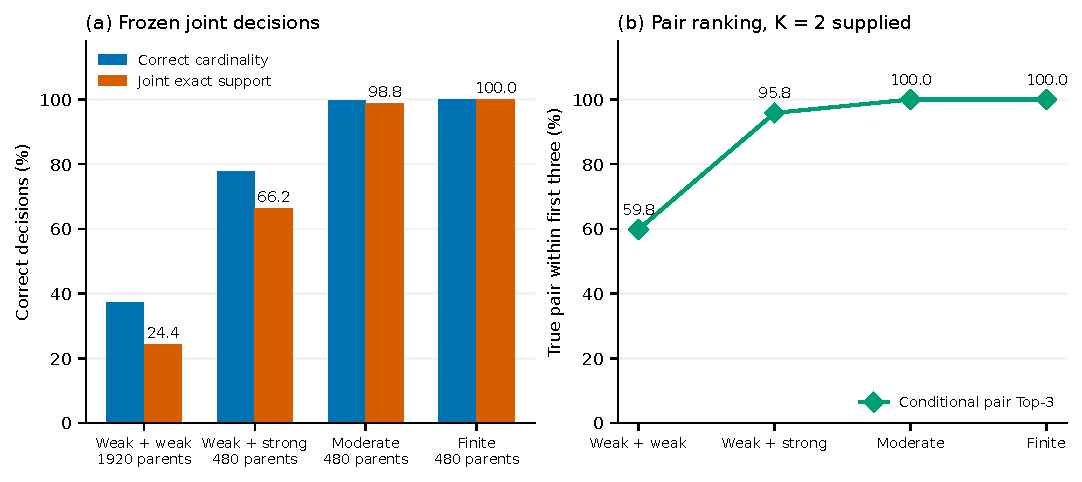
\includegraphics[width=.93\textwidth]{figures/generated/narrative_resolution.pdf}
\caption{The resolution limit behind the attribution problem. The frozen 137-hypothesis load bank increasingly recovers both cardinality and exact support as event strength increases. Weak-pair exact-support Top-1 is much lower than finite-pair Top-1. Cardinality means choosing the correct number of sources; support means choosing their identities. These known-onset batch results explain ambiguity and do not certify R11's causal performance. Repeated noise decisions are grouped by physical trajectory in the archived protocol.}
\label{fig:narrative-resolution}\end{figure*}
